% Fig. 3.3 -- marginal pdf 由 joint pdf 沿一軸積分而得。
% 書稿來源: mathstatch3.tex 第 456 行的 tikzpicture。
%
% 幾何一律照書稿: view={50}{45}、domain 0:4、y domain 0:4、zmax=0.17、
% 三軸都不標刻度; 兩條邊際密度曲線分別畫在 y=4 的後牆與 x=0 的左牆上，
% 各以一個標示與一條牽引線標出 $f_X(x)$ 與 $f_Y(y)$。
%
% 對書稿的四處調整:
%   1. colormap 由 whitegray 改為同色相的墨色濃淡 journalgray (CH3 規格 3.2)。
%   2. samples 由 50 改為 40 (CH3 規格 3.2 所定的產製規格)。
%   3. 兩條邊際密度曲線改為 journalaccent 0.8pt，與灰階曲面分開; 座標軸
%      0.8pt journalink，標示的牽引線走 journalmuted 0.5pt。
%   4. 字級: 書稿的兩個 pin 標示落在 normalsize，其中 $f_{\sssig Y}$ 的下標
%      走 scriptscriptstyle，在 350px 顯示寬之下只有 5.4px，未達 11px 門檻。
%      此處下標一律改為一般下標，並以 \DeclareMathSizes 把 script 級撐到
%      base 的九成; 圖寬同時由 11cm 收到 8.0cm。兩個曲線標示留在 normalsize
%      而未跟著軸名升為 \large，是因為牆面上可放標示的空白只有那麼寬，
%      \large 的標示一定會壓到鉛直稜線或曲線。
%
% 產製 (CH3 規格 3.2 的三維曲面路徑，-O 不可省):
%   latex -interaction=nonstopmode '\def\pgfsysdriver{pgfsys-dvisvgm.def}% Fig. 3.3 -- marginal pdf 由 joint pdf 沿一軸積分而得。
% 書稿來源: mathstatch3.tex 第 456 行的 tikzpicture。
%
% 幾何一律照書稿: view={50}{45}、domain 0:4、y domain 0:4、zmax=0.17、
% 三軸都不標刻度; 兩條邊際密度曲線分別畫在 y=4 的後牆與 x=0 的左牆上，
% 各以一個標示與一條牽引線標出 $f_X(x)$ 與 $f_Y(y)$。
%
% 對書稿的四處調整:
%   1. colormap 由 whitegray 改為同色相的墨色濃淡 journalgray (CH3 規格 3.2)。
%   2. samples 由 50 改為 40 (CH3 規格 3.2 所定的產製規格)。
%   3. 兩條邊際密度曲線改為 journalaccent 0.8pt，與灰階曲面分開; 座標軸
%      0.8pt journalink，標示的牽引線走 journalmuted 0.5pt。
%   4. 字級: 書稿的兩個 pin 標示落在 normalsize，其中 $f_{\sssig Y}$ 的下標
%      走 scriptscriptstyle，在 350px 顯示寬之下只有 5.4px，未達 11px 門檻。
%      此處下標一律改為一般下標，並以 \DeclareMathSizes 把 script 級撐到
%      base 的九成; 圖寬同時由 11cm 收到 8.0cm。兩個曲線標示留在 normalsize
%      而未跟著軸名升為 \large，是因為牆面上可放標示的空白只有那麼寬，
%      \large 的標示一定會壓到鉛直稜線或曲線。
%
% 產製 (CH3 規格 3.2 的三維曲面路徑，-O 不可省):
%   latex -interaction=nonstopmode '\def\pgfsysdriver{pgfsys-dvisvgm.def}% Fig. 3.3 -- marginal pdf 由 joint pdf 沿一軸積分而得。
% 書稿來源: mathstatch3.tex 第 456 行的 tikzpicture。
%
% 幾何一律照書稿: view={50}{45}、domain 0:4、y domain 0:4、zmax=0.17、
% 三軸都不標刻度; 兩條邊際密度曲線分別畫在 y=4 的後牆與 x=0 的左牆上，
% 各以一個標示與一條牽引線標出 $f_X(x)$ 與 $f_Y(y)$。
%
% 對書稿的四處調整:
%   1. colormap 由 whitegray 改為同色相的墨色濃淡 journalgray (CH3 規格 3.2)。
%   2. samples 由 50 改為 40 (CH3 規格 3.2 所定的產製規格)。
%   3. 兩條邊際密度曲線改為 journalaccent 0.8pt，與灰階曲面分開; 座標軸
%      0.8pt journalink，標示的牽引線走 journalmuted 0.5pt。
%   4. 字級: 書稿的兩個 pin 標示落在 normalsize，其中 $f_{\sssig Y}$ 的下標
%      走 scriptscriptstyle，在 350px 顯示寬之下只有 5.4px，未達 11px 門檻。
%      此處下標一律改為一般下標，並以 \DeclareMathSizes 把 script 級撐到
%      base 的九成; 圖寬同時由 11cm 收到 8.0cm。兩個曲線標示留在 normalsize
%      而未跟著軸名升為 \large，是因為牆面上可放標示的空白只有那麼寬，
%      \large 的標示一定會壓到鉛直稜線或曲線。
%
% 產製 (CH3 規格 3.2 的三維曲面路徑，-O 不可省):
%   latex -interaction=nonstopmode '\def\pgfsysdriver{pgfsys-dvisvgm.def}% Fig. 3.3 -- marginal pdf 由 joint pdf 沿一軸積分而得。
% 書稿來源: mathstatch3.tex 第 456 行的 tikzpicture。
%
% 幾何一律照書稿: view={50}{45}、domain 0:4、y domain 0:4、zmax=0.17、
% 三軸都不標刻度; 兩條邊際密度曲線分別畫在 y=4 的後牆與 x=0 的左牆上，
% 各以一個標示與一條牽引線標出 $f_X(x)$ 與 $f_Y(y)$。
%
% 對書稿的四處調整:
%   1. colormap 由 whitegray 改為同色相的墨色濃淡 journalgray (CH3 規格 3.2)。
%   2. samples 由 50 改為 40 (CH3 規格 3.2 所定的產製規格)。
%   3. 兩條邊際密度曲線改為 journalaccent 0.8pt，與灰階曲面分開; 座標軸
%      0.8pt journalink，標示的牽引線走 journalmuted 0.5pt。
%   4. 字級: 書稿的兩個 pin 標示落在 normalsize，其中 $f_{\sssig Y}$ 的下標
%      走 scriptscriptstyle，在 350px 顯示寬之下只有 5.4px，未達 11px 門檻。
%      此處下標一律改為一般下標，並以 \DeclareMathSizes 把 script 級撐到
%      base 的九成; 圖寬同時由 11cm 收到 8.0cm。兩個曲線標示留在 normalsize
%      而未跟著軸名升為 \large，是因為牆面上可放標示的空白只有那麼寬，
%      \large 的標示一定會壓到鉛直稜線或曲線。
%
% 產製 (CH3 規格 3.2 的三維曲面路徑，-O 不可省):
%   latex -interaction=nonstopmode '\def\pgfsysdriver{pgfsys-dvisvgm.def}\input{marginal-pdf-from-surface.tex}'
%   dvisvgm -O -d2 -n -o ../../images/teaching-topics/marginal-pdf-from-surface.svg marginal-pdf-from-surface.dvi

\documentclass[tikz,border=2pt]{standalone}
\usepackage{amsmath}
\usepackage{amssymb}
\usepackage{xcolor}
\usepackage{pgfplots}
\pgfplotsset{compat=1.18}

\definecolor{journalink}{HTML}{1F1C18}
\definecolor{journalmuted}{HTML}{8A7F72}
\definecolor{journalaccent}{HTML}{9C2D2D}

%% 12pt (即 \large) 與 10pt (即 \normalsize) 之下的 script 級各撐到 10pt
%% 與 9pt，使 f 的下標在 350px 顯示寬之下仍在 11px 之上。
\DeclareMathSizes{12}{12}{10}{8}
\DeclareMathSizes{10}{10}{9}{8}

\pgfplotsset{
  colormap={journalgray}{color(0cm)=(white); color(1cm)=(journalink)}
}

\begin{document}
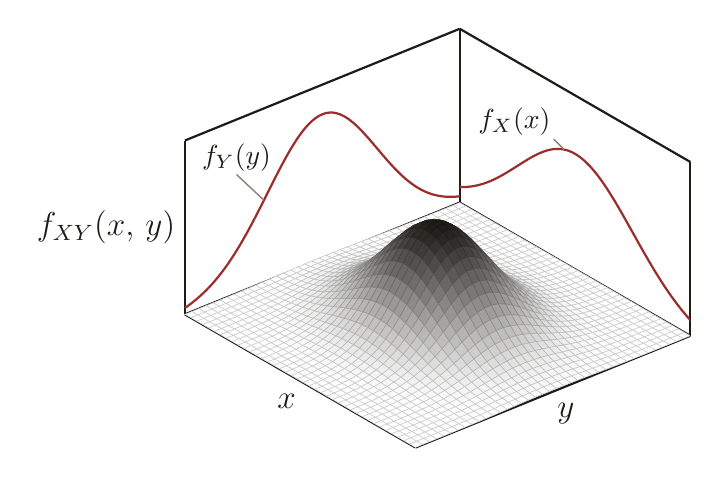
\begin{tikzpicture}[
    declare function={mu1=2;},
    declare function={mu2=2;},
    declare function={sigma1=1;},
    declare function={sigma2=0.8;},
    declare function={normal(\m,\s)=0.4/(2*\s*sqrt(pi))*exp(-(x-\m)^2/(2*\s^2));},
    declare function={bivar(\ma,\sa,\mb,\sb)=
        1/(2*pi*\sa*\sb) * exp(-((x-\ma)^2/\sa^2 + (y-\mb)^2/\sb^2))/2;},
    curvelabel/.style={journalink, font=\normalsize, anchor=east, inner sep=1pt},
    leader/.style={journalmuted, line width=0.5pt}]
\begin{axis}[
    axis line style={journalink, line width=0.8pt},
    colormap name=journalgray,
    width=8.0cm,
    view={50}{45},
    enlargelimits=false,
    grid=minor,
    grid style={journalmuted, line width=0.2pt, opacity=0.4},
    domain=0:4,
    y domain=0:4,
    zmax=0.17,
    samples=40,
    xlabel=$x$,
    ylabel=$y$,
    zlabel={$f_{XY}(x,\,y)$},
    label style={journalink, font=\large},
    xtick=\empty,
    ytick=\empty,
    ztick=\empty,
    zlabel style={rotate=-90, anchor=east},
]
\addplot3[surf, draw=journalink, line width=0.2pt] {bivar(mu1,sigma1,mu2,sigma2)};
%% 兩條邊際密度曲線: 沿一軸積分之後留在後牆與左牆上的那一條
\addplot3[domain=0:4, samples=40, samples y=0, smooth,
          journalaccent, line width=0.8pt] (x,4,{normal(mu1,sigma1)});
\addplot3[domain=0:4, samples=40, samples y=0, smooth,
          journalaccent, line width=0.8pt] (0,x,{normal(mu2,sigma2)});

%% 兩個標示: 書稿用 pin，此處改為位置寫死的節點加牽引線。書稿的 pin 排出來
%% 的位置壓在兩牆相交的鉛直稜線上 (書稿原圖已經擦邊，字級一放大就整個蓋住
%% 稜線)，改為寫死座標才排得開。牽引線的終點取在曲線上:
%%   左牆 (x=0) 的曲線 z = 0.141048 exp(-(y-2)^2/1.28)，y=1.15 處 z=0.0802
%%   後牆 (y=4) 的曲線 z = 0.112838 exp(-(x-2)^2/2)，   x=1.81 處 z=0.1108
%% 位置以像素量過: 標示的墨跡與圖上其他墨跡的最短距離，左邊 0.159cm、
%% 右邊 0.191cm，在 350px 顯示寬之下是 6.5px 與 7.9px。
\node[curvelabel] (fY) at (axis cs:0,1.30,0.118) {$f_{Y}(y)$};
\draw[leader] (fY.south) -- (axis cs:0,1.15,0.0802);
\node[curvelabel] (fX) at (axis cs:1.63,4,0.132) {$f_{X}(x)$};
\draw[leader] (fX.south east) -- (axis cs:1.81,4,0.1108);
\end{axis}
\end{tikzpicture}
\end{document}
'
%   dvisvgm -O -d2 -n -o ../../images/teaching-topics/marginal-pdf-from-surface.svg marginal-pdf-from-surface.dvi

\documentclass[tikz,border=2pt]{standalone}
\usepackage{amsmath}
\usepackage{amssymb}
\usepackage{xcolor}
\usepackage{pgfplots}
\pgfplotsset{compat=1.18}

\definecolor{journalink}{HTML}{1F1C18}
\definecolor{journalmuted}{HTML}{8A7F72}
\definecolor{journalaccent}{HTML}{9C2D2D}

%% 12pt (即 \large) 與 10pt (即 \normalsize) 之下的 script 級各撐到 10pt
%% 與 9pt，使 f 的下標在 350px 顯示寬之下仍在 11px 之上。
\DeclareMathSizes{12}{12}{10}{8}
\DeclareMathSizes{10}{10}{9}{8}

\pgfplotsset{
  colormap={journalgray}{color(0cm)=(white); color(1cm)=(journalink)}
}

\begin{document}
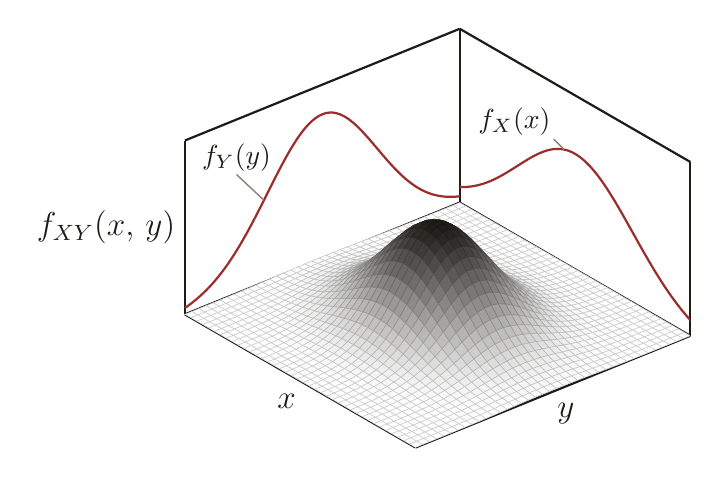
\begin{tikzpicture}[
    declare function={mu1=2;},
    declare function={mu2=2;},
    declare function={sigma1=1;},
    declare function={sigma2=0.8;},
    declare function={normal(\m,\s)=0.4/(2*\s*sqrt(pi))*exp(-(x-\m)^2/(2*\s^2));},
    declare function={bivar(\ma,\sa,\mb,\sb)=
        1/(2*pi*\sa*\sb) * exp(-((x-\ma)^2/\sa^2 + (y-\mb)^2/\sb^2))/2;},
    curvelabel/.style={journalink, font=\normalsize, anchor=east, inner sep=1pt},
    leader/.style={journalmuted, line width=0.5pt}]
\begin{axis}[
    axis line style={journalink, line width=0.8pt},
    colormap name=journalgray,
    width=8.0cm,
    view={50}{45},
    enlargelimits=false,
    grid=minor,
    grid style={journalmuted, line width=0.2pt, opacity=0.4},
    domain=0:4,
    y domain=0:4,
    zmax=0.17,
    samples=40,
    xlabel=$x$,
    ylabel=$y$,
    zlabel={$f_{XY}(x,\,y)$},
    label style={journalink, font=\large},
    xtick=\empty,
    ytick=\empty,
    ztick=\empty,
    zlabel style={rotate=-90, anchor=east},
]
\addplot3[surf, draw=journalink, line width=0.2pt] {bivar(mu1,sigma1,mu2,sigma2)};
%% 兩條邊際密度曲線: 沿一軸積分之後留在後牆與左牆上的那一條
\addplot3[domain=0:4, samples=40, samples y=0, smooth,
          journalaccent, line width=0.8pt] (x,4,{normal(mu1,sigma1)});
\addplot3[domain=0:4, samples=40, samples y=0, smooth,
          journalaccent, line width=0.8pt] (0,x,{normal(mu2,sigma2)});

%% 兩個標示: 書稿用 pin，此處改為位置寫死的節點加牽引線。書稿的 pin 排出來
%% 的位置壓在兩牆相交的鉛直稜線上 (書稿原圖已經擦邊，字級一放大就整個蓋住
%% 稜線)，改為寫死座標才排得開。牽引線的終點取在曲線上:
%%   左牆 (x=0) 的曲線 z = 0.141048 exp(-(y-2)^2/1.28)，y=1.15 處 z=0.0802
%%   後牆 (y=4) 的曲線 z = 0.112838 exp(-(x-2)^2/2)，   x=1.81 處 z=0.1108
%% 位置以像素量過: 標示的墨跡與圖上其他墨跡的最短距離，左邊 0.159cm、
%% 右邊 0.191cm，在 350px 顯示寬之下是 6.5px 與 7.9px。
\node[curvelabel] (fY) at (axis cs:0,1.30,0.118) {$f_{Y}(y)$};
\draw[leader] (fY.south) -- (axis cs:0,1.15,0.0802);
\node[curvelabel] (fX) at (axis cs:1.63,4,0.132) {$f_{X}(x)$};
\draw[leader] (fX.south east) -- (axis cs:1.81,4,0.1108);
\end{axis}
\end{tikzpicture}
\end{document}
'
%   dvisvgm -O -d2 -n -o ../../images/teaching-topics/marginal-pdf-from-surface.svg marginal-pdf-from-surface.dvi

\documentclass[tikz,border=2pt]{standalone}
\usepackage{amsmath}
\usepackage{amssymb}
\usepackage{xcolor}
\usepackage{pgfplots}
\pgfplotsset{compat=1.18}

\definecolor{journalink}{HTML}{1F1C18}
\definecolor{journalmuted}{HTML}{8A7F72}
\definecolor{journalaccent}{HTML}{9C2D2D}

%% 12pt (即 \large) 與 10pt (即 \normalsize) 之下的 script 級各撐到 10pt
%% 與 9pt，使 f 的下標在 350px 顯示寬之下仍在 11px 之上。
\DeclareMathSizes{12}{12}{10}{8}
\DeclareMathSizes{10}{10}{9}{8}

\pgfplotsset{
  colormap={journalgray}{color(0cm)=(white); color(1cm)=(journalink)}
}

\begin{document}
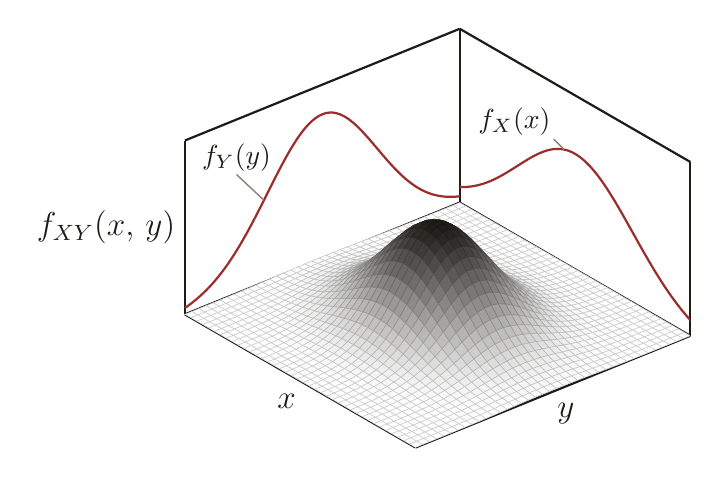
\begin{tikzpicture}[
    declare function={mu1=2;},
    declare function={mu2=2;},
    declare function={sigma1=1;},
    declare function={sigma2=0.8;},
    declare function={normal(\m,\s)=0.4/(2*\s*sqrt(pi))*exp(-(x-\m)^2/(2*\s^2));},
    declare function={bivar(\ma,\sa,\mb,\sb)=
        1/(2*pi*\sa*\sb) * exp(-((x-\ma)^2/\sa^2 + (y-\mb)^2/\sb^2))/2;},
    curvelabel/.style={journalink, font=\normalsize, anchor=east, inner sep=1pt},
    leader/.style={journalmuted, line width=0.5pt}]
\begin{axis}[
    axis line style={journalink, line width=0.8pt},
    colormap name=journalgray,
    width=8.0cm,
    view={50}{45},
    enlargelimits=false,
    grid=minor,
    grid style={journalmuted, line width=0.2pt, opacity=0.4},
    domain=0:4,
    y domain=0:4,
    zmax=0.17,
    samples=40,
    xlabel=$x$,
    ylabel=$y$,
    zlabel={$f_{XY}(x,\,y)$},
    label style={journalink, font=\large},
    xtick=\empty,
    ytick=\empty,
    ztick=\empty,
    zlabel style={rotate=-90, anchor=east},
]
\addplot3[surf, draw=journalink, line width=0.2pt] {bivar(mu1,sigma1,mu2,sigma2)};
%% 兩條邊際密度曲線: 沿一軸積分之後留在後牆與左牆上的那一條
\addplot3[domain=0:4, samples=40, samples y=0, smooth,
          journalaccent, line width=0.8pt] (x,4,{normal(mu1,sigma1)});
\addplot3[domain=0:4, samples=40, samples y=0, smooth,
          journalaccent, line width=0.8pt] (0,x,{normal(mu2,sigma2)});

%% 兩個標示: 書稿用 pin，此處改為位置寫死的節點加牽引線。書稿的 pin 排出來
%% 的位置壓在兩牆相交的鉛直稜線上 (書稿原圖已經擦邊，字級一放大就整個蓋住
%% 稜線)，改為寫死座標才排得開。牽引線的終點取在曲線上:
%%   左牆 (x=0) 的曲線 z = 0.141048 exp(-(y-2)^2/1.28)，y=1.15 處 z=0.0802
%%   後牆 (y=4) 的曲線 z = 0.112838 exp(-(x-2)^2/2)，   x=1.81 處 z=0.1108
%% 位置以像素量過: 標示的墨跡與圖上其他墨跡的最短距離，左邊 0.159cm、
%% 右邊 0.191cm，在 350px 顯示寬之下是 6.5px 與 7.9px。
\node[curvelabel] (fY) at (axis cs:0,1.30,0.118) {$f_{Y}(y)$};
\draw[leader] (fY.south) -- (axis cs:0,1.15,0.0802);
\node[curvelabel] (fX) at (axis cs:1.63,4,0.132) {$f_{X}(x)$};
\draw[leader] (fX.south east) -- (axis cs:1.81,4,0.1108);
\end{axis}
\end{tikzpicture}
\end{document}
'
%   dvisvgm -O -d2 -n -o ../../images/teaching-topics/marginal-pdf-from-surface.svg marginal-pdf-from-surface.dvi

\documentclass[tikz,border=2pt]{standalone}
\usepackage{amsmath}
\usepackage{amssymb}
\usepackage{xcolor}
\usepackage{pgfplots}
\pgfplotsset{compat=1.18}

\definecolor{journalink}{HTML}{1F1C18}
\definecolor{journalmuted}{HTML}{8A7F72}
\definecolor{journalaccent}{HTML}{9C2D2D}

%% 12pt (即 \large) 與 10pt (即 \normalsize) 之下的 script 級各撐到 10pt
%% 與 9pt，使 f 的下標在 350px 顯示寬之下仍在 11px 之上。
\DeclareMathSizes{12}{12}{10}{8}
\DeclareMathSizes{10}{10}{9}{8}

\pgfplotsset{
  colormap={journalgray}{color(0cm)=(white); color(1cm)=(journalink)}
}

\begin{document}
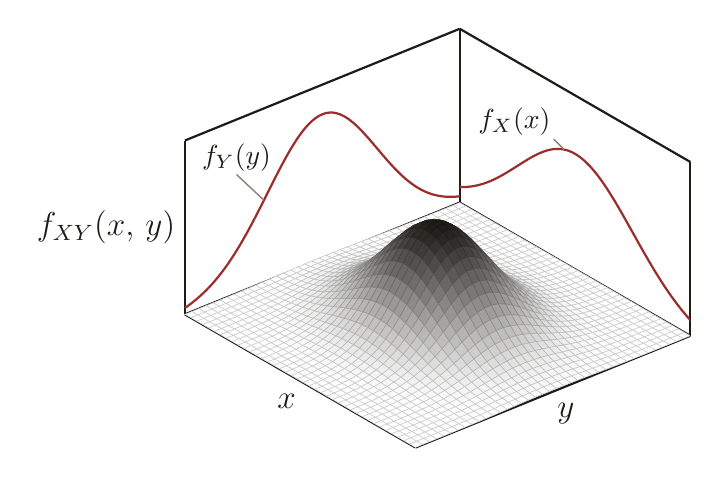
\begin{tikzpicture}[
    declare function={mu1=2;},
    declare function={mu2=2;},
    declare function={sigma1=1;},
    declare function={sigma2=0.8;},
    declare function={normal(\m,\s)=0.4/(2*\s*sqrt(pi))*exp(-(x-\m)^2/(2*\s^2));},
    declare function={bivar(\ma,\sa,\mb,\sb)=
        1/(2*pi*\sa*\sb) * exp(-((x-\ma)^2/\sa^2 + (y-\mb)^2/\sb^2))/2;},
    curvelabel/.style={journalink, font=\normalsize, anchor=east, inner sep=1pt},
    leader/.style={journalmuted, line width=0.5pt}]
\begin{axis}[
    axis line style={journalink, line width=0.8pt},
    colormap name=journalgray,
    width=8.0cm,
    view={50}{45},
    enlargelimits=false,
    grid=minor,
    grid style={journalmuted, line width=0.2pt, opacity=0.4},
    domain=0:4,
    y domain=0:4,
    zmax=0.17,
    samples=40,
    xlabel=$x$,
    ylabel=$y$,
    zlabel={$f_{XY}(x,\,y)$},
    label style={journalink, font=\large},
    xtick=\empty,
    ytick=\empty,
    ztick=\empty,
    zlabel style={rotate=-90, anchor=east},
]
\addplot3[surf, draw=journalink, line width=0.2pt] {bivar(mu1,sigma1,mu2,sigma2)};
%% 兩條邊際密度曲線: 沿一軸積分之後留在後牆與左牆上的那一條
\addplot3[domain=0:4, samples=40, samples y=0, smooth,
          journalaccent, line width=0.8pt] (x,4,{normal(mu1,sigma1)});
\addplot3[domain=0:4, samples=40, samples y=0, smooth,
          journalaccent, line width=0.8pt] (0,x,{normal(mu2,sigma2)});

%% 兩個標示: 書稿用 pin，此處改為位置寫死的節點加牽引線。書稿的 pin 排出來
%% 的位置壓在兩牆相交的鉛直稜線上 (書稿原圖已經擦邊，字級一放大就整個蓋住
%% 稜線)，改為寫死座標才排得開。牽引線的終點取在曲線上:
%%   左牆 (x=0) 的曲線 z = 0.141048 exp(-(y-2)^2/1.28)，y=1.15 處 z=0.0802
%%   後牆 (y=4) 的曲線 z = 0.112838 exp(-(x-2)^2/2)，   x=1.81 處 z=0.1108
%% 位置以像素量過: 標示的墨跡與圖上其他墨跡的最短距離，左邊 0.159cm、
%% 右邊 0.191cm，在 350px 顯示寬之下是 6.5px 與 7.9px。
\node[curvelabel] (fY) at (axis cs:0,1.30,0.118) {$f_{Y}(y)$};
\draw[leader] (fY.south) -- (axis cs:0,1.15,0.0802);
\node[curvelabel] (fX) at (axis cs:1.63,4,0.132) {$f_{X}(x)$};
\draw[leader] (fX.south east) -- (axis cs:1.81,4,0.1108);
\end{axis}
\end{tikzpicture}
\end{document}
